\chapter{Characterizing Radio Energy Usage of Smartphones in Cellular Networks} 
\label{chap:power}

Smartphones with cellular data access have become increasingly popular across the globe, with the wide deployment of 3G and emerging LTE~\cite{3gpp.lte} networks, and a plethora of applications of all kinds. Cellular networks are typically characterized by limited radio resources and significant device power consumption for network communications. The battery capacity of smartphones cannot be easily improved due to physical constraints in size and weight. Hence, battery life remains a key determinant of end-user experience. Given the limited radio resources in these networks and device battery capacity constraints, optimizing the usage of these resources is critical for cellular carriers and application developers. Specifically, radio power is reported to be 1/3 to 1/2 of the total device power~\cite{mobisys.aro}, and in this chapter, we first devise a systematic way to characterize smartphone radio energy usage given packet traces as input and then we discuss our analysis results with real user traces.

\nsection{Power Measurement Methodology}
\label{sec:power.method}

Similar to previous studies~\cite{imc.3g, codes.powertutor}, we use Monsoon power monitor~\cite{monsoon} as power input for our device measuring power traces at the same time. The power trace contains two fields, timestamp and average instant power, and the sampling rate is 5000Hz. The test device is an HTC phone with LTE data plan from a cellular ISP. It has 768 MB RAM memory and 1 GHz Qualcomm MSM8655 CPU, running Android 2.2.1. We remove the battery and connect $\oplus$ and $\ominus$ pins of the power monitor to device's $\oplus$ and $\ominus$ pins, respectively. By enabling $V_{out}$ with the voltage of 3.7V, the device boots properly and the power monitor records the total power traces consumed by the device. Another tricky part for our setup is that, the back cover of our test device, HTC Thunderbolt, must remain attached firmly, otherwise, if it is pried off the device, LTE session is terminated and 1xRTT session is started. This is because part of the LTE antenna circuit lies inside the back cover~\cite{thunderbolt}. In the end, we let the wires going out of the back cover through the hole of earplugs.

%In Section~\ref{sec:background.power},  Figure~\ref{fig:trace.all} and Figure~\ref{fig:trace.zoom} visualize one such power measurement in LTE network.
We share the same observation with previous study~\cite{codes.powertutor} that screen plays an important role in device power consumption, \ie with screen 100\% on, the UE idle power is 847.15mW compared with 11.36mW with screen off. For all measurements, we keep the test application running in the background with screen completely off to minimize power noise, unless UI interactions are required and screen should be kept on, \ie measuring power for browser. In this case, we subtract screen power from the total, with slightly increased noise. All experiments are repeated at least 5 times to reduce measurement error.

To measure state transition power levels, UE keeps a long-lived TCP connection with the server and packet traces are collected to make sure there is no background traffic. In order to trigger state promotions, we make the device idle for sufficient time, \eg 30 seconds, and then send a packet from server to client. UE remains idle afterwards and demotes to idle state in the end, and the power trace covers the full tail.

\nsection{Smartphone Power Model}

In Section~\ref{sec:bkg.rrc}, we have discussed the radio resource control mechanisms in cellular network. In fact, RRC state machine is the key factor for determining the UE power consumption for both 3G and LTE 4G networks.

In this section, we take LTE network as a sample and illustrate the power traces of our test Android smartphone in a commercial LTE network based on local experiments. We observe that network activities match the corresponding state transitions indicated by different power levels.

\begin{figure}[t]
\centering
\IG{figures/mobisys12/trace_all.eps} \\
\ncaption{Power states of LTE}
\label{fig:trace.all}
\end{figure}

%So the plot of power traces in Figure 3 consists of dots of readings and may be >>594mW. During the DRX in RRC_IDLE, the actual power curve is something like a "n" shape curve (an increase period, a fluctuating top, and a decrease period). The average of the whole on period is 594mW, but the pikes inside the on period can be >>594mW. Those spikes have very minor effect in the energy calculation, but they are very obvious to see in the power trace figure.

Figure~\ref{fig:trace.all} shows the power trace of uploading at the speed of 1Mpbs for 10 seconds. With screen off, the energy is mostly consumed by the radio interfaces, as the power level is less than 20mW before $t_1$. At $t_1$, the application sends a TCP {\sf SYN} packet triggering \RI to \RC promotion, and the application waits for $T_{pro}$ until starting data transfer at $t_2$. Between $t_2$ and $t_3$, depending on the instant data rate, the power level fluctuates. We notice the power level during fast data transfer is significantly higher than the base power in \RC, which motivates us to incorporate data rates into our LTE power model. After the data transfer completes at $t_3$, the device remains in \RC for a fixed tail time $T_{tail}$, until $t_4$, when the device goes back to \RI. The periodicity of DRX between $t_3$ and $t_4$ is not obvious due to limited sample rate.

%If there is any data sent or received between $t_3$ and $t_4$, the tail timer gets reset and a new tail starts.

\begin{figure}[h]
\centering
\IG{figures/mobisys12/trace_zoom.eps} \\
\ncaption{Zoom-in view in \RC}
\label{fig:trace.zoom}
\end{figure}

Figure~\ref{fig:trace.zoom} is a 125$\times$ zoom-in view of Figure~\ref{fig:trace.all}'s tail, which clearly illustrates DRX activity in \RC~mode. The device activates its receivers to listen to downlink control channel. If downlink traffic is found awaiting, the device goes into Continuous Reception model; otherwise, the device goes into a dormant state without continuously checking downlink control channel, though still remaining in \RC~mode. The spikes appearing every 40 ms in Figure~\ref{fig:trace.zoom} match the on period of DRX in \RC.



\nsection{Power Model Construction}
\label{sec:power.model}
This section summarizes the construction of the new LTE power model, as well as the 3G and WiFi model measured from the same LTE phone. We then compare energy efficiency in bulk data transfer for different networks and validate LTE power model in the end.

\begin{table}[t]
\begin{center}
\begin{tabular}{|c|c|c|c|c|}\hline
 & Power$^\star$ & Duration & Periodicity\\
 & (mW) & (ms) & (ms)\\\hline\hline
Screen off (base) & 11.4$\pm$0.4 & N/A & N/A\\\hline
Screen 100\% on & 847.2$\pm$2.7 & N/A & N/A\\\hline\hline
 
\MR{LTE promotion} & \MR{1210.7$\pm$85.6} & $T_{pro}$: & \MR{N/A} \\
 &  &  260.1$\pm$15.8 & \\\hline
%it's not continuous reception since there is 40ms DRX
LTE Short DRX On & \MR{1680.2$\pm$15.7} & $T_{on}$: & $T_{ps}$:\\
\RC & & 1.0$\pm$0.1 & 20.0$\pm$0.1 \\\hline
LTE Long DRX On & \MR{1680.1$\pm$14.3} & $T_{on}$: & $T_{pl}$:\\
\RC & & 1.0$\pm$0.1 & 40.1$\pm$0.1 \\\hline
\MR{LTE tail base} & \MR{1060.0$\pm$3.3} & $T_{tail}$: & \MR{N/A} \\
 &  & 11576.0$\pm$26.1 & \\\hline
LTE DRX On & \MR{594.3$\pm$8.7} & $T_{oni}$: & $T_{pi}$:\\
\RI &  & 43.2$\pm$1.5 & 1280.2$\pm$7.1\\\hline\hline

3G promotion & 659.4$\pm$40.4 & 582.1$\pm$79.5 & N/A \\\hline
3G DCH tail base & 803.9$\pm$5.9 & 8088.2$\pm$149.6 & N/A \\\hline
3G FACH tail base & 601.3$\pm$6.4 & 824.2$\pm$148.1 & N/A \\\hline
3G DRX (idle) & 374.2$\pm$13.7 & 55.4$\pm$1.5 & 5112.4$\pm$37.7 \\\hline\hline

WiFi promotion & 124.4$\pm$2.6 & 79.1$\pm$15.1 & N/A \\\hline
WiFi tail base & 119.3$\pm$2.5 & 238.1$\pm$9.2 & N/A \\\hline
WiFi beacon (idle) & 77.2$\pm$1.1 & 7.6$\pm$0.1 & 308.2$\pm$1.0 \\\hline
\end{tabular}
\ncaption{LTE, 3G, and WiFi power model}
\label{tab:power}
\begin{tabular}{l}
\\{$^\star$All power readings in this table include the base power (screen off),}\\
{~~which has negligible impact on total energy.}
\end{tabular}
\end{center}
\end{table}

\nsubsection{Power model for RRC and DRX}
\label{sec:power.rrc}

With the experimental setup described in Section~\ref{sec:power.method}, we measure power model for LTE, 3G, and WiFi on the LTE phone, summarized in Table~\ref{tab:power}. The LTE parameter values are validated by the network-based measurement in Section~\ref{sec:net.sm}\comment{update reference}. For simplicity, we ignore the WiFi AP scanning and association, assuming UE is already connected with an AP.

First, we observe that LTE reduces the promotion delay ($T_{pro}$) from 3G's 582.06ms to 260.13ms. However, the power level is almost doubled, \ie 1210.74mW (LTE) v.s. 659.43mW (3G). WiFi has the most lightweight state promotion with smaller $T_{pro}$ and much lower power level.

Secondly, LTE appears to have longest tail (11.576 seconds) with highest tail base power (1060.04 mW). Summing up DCH and FACH tail, 3G's total tail time (8.9 seconds) is smaller than LTE's $T_{tail}$ of 11.6 seconds. Even 3G DCH's tail base power is 24.17\% lower than LTE's tail base power, and the gap becomes 25.25\% if we consider LTE DRX in \RC with a high on duration power (1680.20mW). WiFi is much more power efficient, with shorter tail and much lower base power.

We also compare LTE DRX in \RI~with 3G DRX and WiFi beacon in the idle state. LTE has the highest on power and slightly smaller On Duration than 3G, while WiFi has smallest on power and On Duration. The cycle of LTE (1.28 seconds) is in between 3G and WiFi.

Based on these observations, LTE is less energy efficient during idle state and for transferring smaller amount of data. For example, if only one packet is transferred, the energy usage considering both promotion and tail energy for LTE, 3G and WiFi is 12.76J, 7.38J and 0.04J, respectively. One possible reason for LTE's higher power states is that devices must incorporate {\em multiple-input and multiple-output} (MIMO) to support LTE network, \eg the test device we use has 1 transmit antenna and 2 receive antennas, which contributes to higher power consumption.

\begin{figure*}[tp]
\centering
\begin{minipage}[b]{.49\textwidth}
\centering
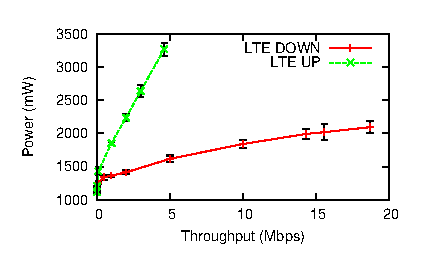
\includegraphics[width=.99\textwidth]{figures/mobisys12/power_tp.eps}
\ncaption{\small Power-throughput curve for LTE network}
\label{fig:power.tp}
\end{minipage}
\begin{minipage}[b]{.49\textwidth}
\centering
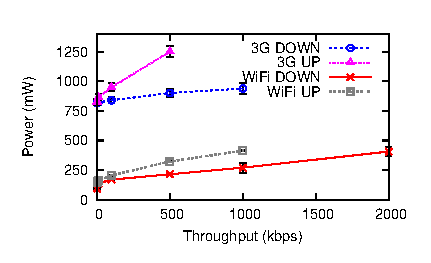
\includegraphics[width=.99\textwidth]{figures/mobisys12/power_tp2.eps}
\ncaption{\small Power-throughput curve for 3G and WiFi}
\label{fig:power.tp2}
\end{minipage}
\end{figure*}

\begin{figure}[t]
\centering
\IG{figures/mobisys12/up_down.eps} \\
\ncaption{Power of simultaneous uplink and downlink transfers}
\label{fig:up.down}
\end{figure}



\nsubsection{Power Model for Data Transfer}
\label{sec:power.updown}
Previous work on 3G UMTS power modeling either treats DCH power state to have a fixed power value~\cite{codes.powertutor, mobisys.aro}, or assumes energy per bit to be the same constant for both uplink and downlink~\cite{imc.tailender}. These assumptions might be reasonable given that 3G has relatively low data rates. However, for LTE, we observe that device power is much higher during high speed data transmission (up to 3300mW for uplink) relative to the base power (1060mW) in \RC, and there is significant difference between downlink and uplink power levels at the same data rate. In this paper, we propose a new comprehensive power model for LTE empirically derived in a commercial LTE network.

We start with measuring device power states with controlled uplink or downlink throughput. The impact of TCP {\sf ACK} packets, which are small in size, is minor, thus ignored.

%TCP uplink data transfer incurs ACK packets in downlink direction, and vise versa. However, the impact of ACK packets is minor, which are smaller and fewer than data packets and the number of ACK packets.

Figures~\ref{fig:power.tp} and~\ref{fig:power.tp2} present the power-throughput curve for LTE, 3G, and WiFi. The curves are limited by the peak data rate we can achieve at the test location.
We observe that for all networks, a linear model fits well for both uplink and downlink. Assume uplink throughput is $t_u$ (Mbps) and downlink throughput is $t_d$ (Mbps), the power level (mW) for uplink is $P_u = \alpha_u t_u + \beta$ and for downlink $P_d = \alpha_d t_d + \beta$.
The best fit parameters are listed in Table~\ref{tab:up.down}.

\begin{table}[t]
\begin{center}
\begin{tabular}{|c|c|c|c|c|}\hline
 & $\alpha_u$ (mW/Mbps) & $\alpha_d$ (mW/Mbps) & $\beta$ (mW) & $\alpha_u/\alpha_d$ \\\hline
LTE & 438.39 & 51.97 & 1288.04 & 8.44\\\hline
3G & 868.98 & 122.12 & 817.88 & 7.12\\\hline
WiFi & 283.17 & 137.01 & 132.86 & 2.07\\\hline
\end{tabular}
\ncaption{Data transfer power model}
\label{tab:up.down}
\end{center}
\end{table}

By looking at $\alpha_u/\alpha_d$, we notice that uplink power increases faster than downlink for all three networks types. This is expected because sending data requires more power than receiving data for wireless data access~\cite{ieee.mimo}. LTE has the largest gap of $\alpha_u/\alpha_d = 8.44$ among three network types. This is largely because $\alpha_d$ for LTE is quite small. For 3G, both $\alpha_u$ and $\alpha_d$ are larger than LTE. $\beta$ is the base power when throughput is 0, with the ranking of LTE $>$ 3G $>$ WiFi. This is consistent with the tail base power comparison in Table~\ref{tab:power}. We notice that $\beta$ is slightly higher than the tail base for all networks types. This is possibly because of the overhead of switching transmitters or receivers into high speed mode.


For simultaneous uplink and downlink transfers, given that transmitters and receivers are separate, we conjecture that the power level (mW) is given by the following formula:
\begin{equation*}
P = \alpha_u t_u + \alpha_d t_d+ \beta
\end{equation*}
To validate this conjecture, we measure the power levels for concurrent uplink and downlink transfers in Figure~\ref{fig:up.down}. Assume total throughput $t = t_u + t_d$ and the ratio of uplink throughput $\epsilon = t_u \big/ t$:
\begin{equation*}
P = \alpha_u t_u + \alpha_d t_d+ \beta = (\alpha_u - \alpha_d)t\epsilon + \alpha_d t + \beta
\end{equation*}
When $t$ is a constant, $P$ grows linearly with $\epsilon$ and the slope is $(\alpha_u - \alpha_d)t$. Figure~\ref{fig:up.down} shows two curves of $t = 1$Mbps and $t = 2$Mbps, both having a strong linear pattern and the slope is less than 5\% off the expected value.


\nsubsection{Energy Efficiency for Bulk Data Transfer}
\label{sec:power.bulk}

\begin{figure}[t]
\centering
\IG{figures/mobisys12/energy_size.eps} \\
\ncaption{Energy per bit for bulk data transfers}
\label{fig:energy.size}
\end{figure}

To compare the power efficiency of different networks in the wild, we use bulk data transfer experiments to measure energy per bit.
Perrucci \etal~\cite{vtc.survey} measure energy per bit for 3G and WiFi with a fixed bulk size. In addition to taking LTE into consideration, we vary the bulk size to cover more possible network usage scenarios. Figure~\ref{fig:energy.size} shows the measured energy per bit in $\mu J / bit$ ($10^{-6} Joule / bit$) with different bulk data size. All data is randomly generated so that there is no chance for caching. We do not include promotion or tail energy but instead focus on data transfer energy. Given that signal strength and peak data rate on wireless networks fluctuates, both affecting energy per bit, our measurement only serves as a sampled view for the energy efficiency of different networks.
%\comment{why cite this study only?  it's the closest to ours?}

First, energy per bit decreases as bulk data size increases, largely because with a small data size, throughput does not reach link capacity due to TCP slow start. We also observe that LTE's energy per bit in downlink is comparable with WiFi, although the absolute power level of LTE is much higher than WiFi. This is due to high downlink throughput for LTE at our test location, even compared with the WiFi network. Similarly, for LTE uplink, it drops from 10$\mu J / bit$ to less than 1$\mu J / bit$ as bulk data size increases. With bulk data size of 10MB, LTE consumes 1.62 times the energy of WiFi for downlink and 2.53 for uplink. With lowest throughput, 3G has the worst energy efficiency for large data transfer, \eg for downloading 10MB data, 3G requires 21.50 times the energy of LTE and 34.77 times the energy of WiFi, and for uplink, 7.97 times of LTE and 20.16 times of WiFi.

%3G and LTE require 34.77 and 1.62 times the energy of WiFi, respectively, and for uplink, 3G/WiFi ratio is 20.16 and LTE/WiFi ratio is 2.53.
%\comment{I thought these numbers are interesting and should be included in the intro: in particular, you should have small transfer (1 packet) vs. bulk transfer energy per bit comparision}

\nsubsection{Power Model Validation}
\label{sec:power.validation}

\begin{table}[h]
\begin{center}
\begin{tabular}{|c|c|c|c|c|}\hline
\MR{App} & Measured & Simulated & \MR{Error}  \\
&energy (J)\footnotemark[1] & energy (J)\footnotemark[1] &\\\hline
Website G\footnotemark[3] & 24.77 & 24.37 & -1.61\% (-2.06\%\footnotemark[2]) \\\hline
Website Y\footnotemark[3] & 31.84 & 30.08 & -5.53\% (-7.04\%) \\\hline
YouTube & 21.81 & 21.14 & -3.07\% (-4.17\%) \\\hline
NPR News & 24.65 & 24.37 & -1.12\% (-1.70\%) \\\hline
Market & 38.64 & 38.03 & -1.58\% (-3.03\%) \\\hline
\end{tabular}
\\
\begin{tabular}{l}
{$^1$Both measured and simulated energy include tail energy}\\
{$^2$This error is for simulated energy assuming $\alpha_u = \alpha_d = 0$}\\
{$^3$Refer to \S\ref{sec:method.app}\comment{update reference} for the definition of \WG and \WY}\\
\end{tabular}
\ncaption{LTE power model validation}
\label{tab:power.validation}
\end{center}
\end{table}

To validate the LTE power model and the trace-driven simulation (\S\ref{sec:method.sim}), we compare measured energy (measured from the LTE phone) with simulated energy for case study applications. Table~\ref{tab:power.validation} contains the sample application usage scenarios described in \S\ref{sec:method.app}. The error rate is consistently less than 6\%, with the largest error rate from \WY, which includes heavy JavaScript execution and HTML rendering. Since our power model focuses on radio power and ignores the impact of CPU, for \WY, the total energy usage is slightly underestimated. 
%As we observe, the impact of non-network components on total energy is minor, except for the excluded screen. 

The error rate is increased if the impact of downlink and uplink throughput is ignored, \ie assuming $\alpha_u = \alpha_d = 0$. However, the increase is not significant, at most 1.5\%. This is because for these web-based applications, network throughput is low due to small object size (\S\ref{sec:app.perf}\comment{update reference}). For other applications, such as video/audio streaming and file download, we expect to see a larger gap in error rate if the impact of downlink/uplink is ignored.

In this section, in addition to comparing energy per bit in bulk data transfer for different networks, we construct a new LTE power model and validate its accuracy, which is the basis for the following analysis.


\nsection{Trace-driven Analysis Methodology}
To compare energy consumption for different networks using real user traces and evaluate the impact of setting LTE parameters, we devise a systematic methodology for trace-driven analysis, which is applied to a comprehensive user trace data set, named \UMICH.

\nsubsection{\UMICH~Data Set for Analysis}

\UMICH~data set is collected from 20 smartphone users for five months, 05/12/2011 $\sim$ 10/12/2011, totaling 118 GB.
These participants consist of undergraduate and graduate students from 8 departments at University of Michigan. The 20 participants are given Motorola Atrix (11 of them) or Samsung Galaxy S smartphones (9 of them) with unlimited voice, text and data plans, all running Android 2.2. As stated in our study consent form, we keep collected data and users' identities strictly confidential\footnote{This user study has been approved by the University of Michigan IRB-HSBS \#HUM00044666.}.
%They are encouraged to take advantage of all the features and services of the phones.

Custom data collection software developed by us are deployed on the 20 smartphones. It continuously runs in the background and collects full packet traces in tcpdump format including both headers and payload. Both cellular and Wi-Fi traces are collected without any sampling performed. The data collector incurs no more than 15\% of CPU overhead, although the overhead is much lower when the throughput is low (\eg less than 200 kbps).

We also build a data uploader that uploads the data to our server when the phone is idle as indicated by low network throughput. The upload is suspended by detected network activity of user applications. The entire data collection and uploading process is transparent to the users.

\nsubsection{Trace-driven Modeling Methodology}
\label{sec:method.sim}
We build a network model and power model analysis framework for the trace-driven analysis, totaling about 8,000 lines of code in C++.

%\paragraph{Trace parser} is for reading binary packet trace files in libpcap~\cite{tcpdump} format. We use a simple data structure that only store the most important fields of a packet and reduce the total data size from 118GB to under 16GB which fits into memory. However, the trace parser can be easily improved to support larger data size that is impossible to be fully loaded into memory, given that it parses packets sequentially and sorting packets is easy with proper file structure design during data collection stage. The output of trace parser is an array of packets with ascending timestamps.

\paragraph{Network model simulator} takes the binary packet trace files in libpcap~\cite{tcpdump} format and preprocesses the data following the same methodology as previous study~\cite{imc.3g}, for the purpose of removing existing delays imposed by state promotions and extracting the actual traffic patterns, \eg for the purposing of simulating the trace in another network. It then applies a specific network model to the processed traces and adjusts timestamps for some packets, since different network models have different delay behavior due to state machine differences. There are two reasons for a packet's timestamp to be adjusted, promotion delay and DRX waiting time.  We use the same methodology to adjust timestamp for promotion delay as previous study~\cite{imc.3g}. In LTE network, if there is no packet for over $T_{tail}$ time, when the next packet $P$ arrives, an extra delay $T_{pro}$ is inserted before $P$. In terms of DRX waiting time, if a downlink packet $P'$ comes at time $T_{P'}$ and UE is in DRX mode, either in \RC or \RI, there is no DRX waiting time if $P'$ arrives inside any DRX on duration; otherwise, $P'$ would experience an extra delay of $T_n - T_{P'}$, where $T_n$ is the start time of the next DRX on duration after $T_{P'}$. The parameters for different network models are listed in Table~\ref{tab:power}, obtained from local experiments. We also empirically assume that UE goes into complete sleep with 0 power usage after being idle for $T_{tail2}$ (1 minute). Notice that $T_{tail2}$ is not actually observed in our experiments and is only used to bound the total idle energy and simplify our analysis.

%, UE should have been in \RI already upon $P$'s arrival, and hence a promotion to \RC is triggered by $P$. A
%\comment{the original trace doesn't contain any such delays? because it's a WiFi trace? please explain.}
%If one packet within a TCP flow is delayed in the simulator, \eg a TCP SYN packet, all subsequent packets dependent on it in that flow are delayed. Similarly, if one flow gets delayed in a web transaction, \eg downloading {\sf index.html} when loading a website, all other flows dependent on it get delayed as well. Arguably, once the user gets delayed on one application, following applications usage might be delayed as well, which however it not always true.
%Given the inherent difficulty of understanding the inter-flow dependency in the user traces, in the simulation, we assume for simplicity that, if one packet gets delayed, all future packets of this user get the same delay.

The output of network model simulator is an array of packets with adjusted timestamps, in ascending order, as well as the RRC and DRX states of UE at any time.

\paragraph{Power model simulator} takes the output of network model simulator and calculates the energy consumption based on the power model, detailed in Section~\ref{sec:power.model}. We break down the total energy into four components: {\em promotion}, {\em data transfer}, {\em tail}, and {\em idle}.

For promotion energy, both promotion delay $T_{pro}$ and average promotion power $P_{pro}$ are fixed. If a trace includes $N$ promotions, promotion energy is given by $NT_{pro}P_{pro}$.

For idle energy in \RI, assume that DRX cycle is $T_{pi}$ (with base power $P_{b}$) and on duration is $T_{oni}$ (with on power $P_{oni}$), energy consumption of an duration of $t_{idle}$ is given by
\begin{equation*}
\lfloor \frac{t_{idle}}{T_{pi}} \rfloor \Big(T_{oni} P_{oni} + (T_{pi} - T_{oni}) P_{b}\Big) + E_{res}
\end{equation*}
where the remaining energy $E_{res}$ can be calculated as
\[E_{res} = \left\{ 
\begin{array}{l l}
T_{res}P_{oni} & \mbox{if$\quad T_{res} \le T_{oni}$}\\
T_{oni}P_{oni} + (T_{res}-T_{oni}) P_{b} & \mbox{if$\quad T_{res} > T_{oni}$}\\ 
\end{array} \right. \]
with
\begin{equation*}
T_{res} = t_{idle} - T_{pi}\lfloor \frac{t_{idle} }{T_{pi}} \rfloor
\end{equation*}

Tail energy is more complex for LTE since \RC has three modes as in Figure~\ref{fig:sm}\comment{update reference}, while 3G and WiFi do not have DRX in connected mode. We simulate the transitions among Continuous Reception, Short DRX and Long DRX to calculate tail energy, in a similar way of idle energy calculation. Note that we only count tail energy when the tail is complete, otherwise, the energy is considered as data transfer energy, \ie if one packet $P$ is observed before UE demotes to \RI at the end of the tail, the energy between $P$ and the previous packet is still considered as data transfer energy.
 
For data transfer energy, we propose a novel model. Assume uplink throughput is $t_u$ (Mbps) and downlink throughput is $t_d$ (Mbps), the instant power level (mW) of UE is
\begin{equation*}
\label{for:updown}
P = \alpha_u t_u + \alpha_d t_d+ \beta
\end{equation*}
Validation of this formula is in \S\ref{sec:power.updown}. 
%Given that packet header length (at most 52 bytes with TCP header 32 bytes and IP header 20 bytes) is much smaller than MTU (1428 bytes for our setup), and that TCP ACK packets are much smaller and typically fewer than data packets, we simply consider payload throughput in our power model, without considering header length and ACK packets.
We simply consider payload throughput in our power model, without considering header length and {\sf ACK} packets due their small impact. Since TCP instant throughput changes frequently, in order to accurately estimate the instant power levels, we divide the trace into small time windows with size $W$ seconds and within each window, throughput $t_u$ and $t_d$ are calculated, which determine the power $P$. $W$ is set to be 1 second empirically in our setup and the total energy is not sensitive to the choice of $W$ as long as $W$ is larger than a few RTTs and smaller than most flow durations. 


\nsection{User trace based tradeoff analysis}
\label{sec:simulation}

In this section, we apply the LTE power model to \UMICH data set and compare energy efficiency with 3G and WiFi, with detailed break down of the total energy. We then study the tradeoff of configuring different LTE parameters via our analysis framework.

\subsection{Energy efficiency comparison}
\label{sec:sim.total}

\begin{figure}[t]
\centering
\IG{figures/mobisys12/energy_ratio.eps} \\
\ncaption{Power model simulation: energy ratio}
\label{fig:energy.ratio}
\end{figure}

%Given that LTE has comparable RTT with WiFi as discussed in \S\ref{sec:net}, we use WiFi traces in \UMICH~data set to simulate the LTE model. We also simulate 3G and WiFi model with 3G and WiFi traces, respectively. Assume the total payload of 3G traces in \UMICH~data set is $S_{3g}$ bits, and $S_{wifi}$ for WiFi traces. Also assume that the simulated energy usage for LTE, WiFi and 3G power model is $E_{lte}$, $E_{wifi}$ and $E_{3g}$, respectively, the energy ratio of LTE/WiFi is defined as $(E_{lte}/S_{wifi})/(E_{wifi}/S_{wifi})=E_{lte}/E_{wifi}$, and that for 3G/WiFi is calculated as $(E_{3g}/S_{3g})/(E_{wifi}/S_{wifi})$. 

We use the \UMICH data set to simulate the LTE, WiFi and 3G model. Assume that the simulated energy usage for LTE, WiFi and 3G power model is $E_{lte}$, $E_{wifi}$ and $E_{3g}$, respectively, the energy ratio of LTE/WiFi is defined as $E_{lte}/E_{wifi}$, and that for 3G/WiFi is calculated as $E_{3g}/E_{wifi}$. With the same traces, we can make fair comparison among different power models to understand their energy efficiency.

In Figure~\ref{fig:energy.ratio}, we compare the energy efficiency of different networks for the 20 users both individually and in aggregate (summing up for all users). We first observe that LTE power model consumes significantly more energy than WiFi. The ratio of LTE/WiFi ranges from 16.9 to 28.9 and the aggregate ratio for all users is 23.0. Notice that the gap between LTE and WiFi is larger compared with the bulk data transfer experiments in \S\ref{sec:power.bulk}. This is because, for bulk data transfer, LTE's high throughput could compensate the low energy efficiency, compared with real traces, which do not saturate the link capacity. Second, for 3G/WiFi ratio, the range is between 10.8 and 18.0, and in aggregate, 3G/WiFi ratio is 14.6, lower than LTE. In summary, the energy efficiency for LTE is lower than 3G, with WiFi having a much higher energy efficiency. Notice that in this work, we do not consider AP association energy for WiFi networks due to the lack of such information, so $E_{wifi}$ is an underestimate. However, we believe that AP association does not happen very often and the impact is not significant.

%We observe that for some users, their 3G traces include more small data transfers than average, which increase the energy per bit for their 3G energy.
%In summary, there is non-negligible application usage differences among different users, even between the same user in 3G network and in WiFi network, which results in variation in energy comparison among different networks. In aggregate, energy per bit for LTE is as high as 24.2 times of WiFi, and 3G is 12.8 times of WiFi.

\subsection{Energy consumption break down}
\label{sec:sim.breakdown}

\begin{figure}[t]
\centering
\IG{figures/mobisys12/energy_breakdown.eps} \\
\ncaption{Break down of energy usage in analysis}
\label{fig:energy.breakdown}
\end{figure}

\begin{figure*}[tp]
\centering
	\begin{minipage}[b]{.49\textwidth}
\centering
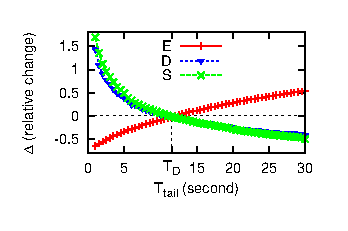
\includegraphics[width=.99\textwidth]{figures/mobisys12/Ta2i.eps}
\ncaption{\small Impact of the LTE tail timer $T_{tail}$}
\label{fig:ta2i}
	\end{minipage}
	\begin{minipage}[b]{.49\textwidth}
\centering
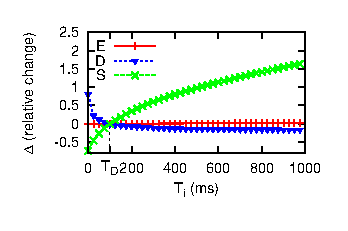
\includegraphics[width=.99\textwidth]{figures/mobisys12/T1.eps}
\ncaption{\small Impact of DRX inactivity timer $T_i$}
\label{fig:t1}
	\end{minipage}
	\begin{minipage}[b]{.49\textwidth}
\centering
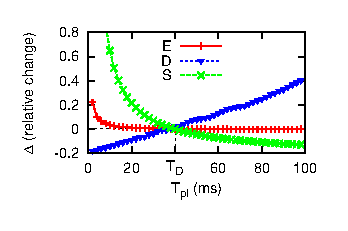
\includegraphics[width=.99\textwidth]{figures/mobisys12/Tpl.eps}
\ncaption{\small Impact of the DRX cycle in \RC~($T_{pl}$)}
\label{fig:tpl}
	\end{minipage}
	\begin{minipage}[b]{.49\textwidth}
\centering
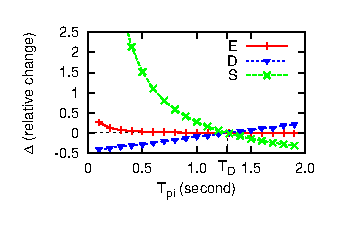
\includegraphics[width=.99\textwidth]{figures/mobisys12/Tpi.eps}
\ncaption{\small Impact of DRX cycle in \RI~($T_{pi}$)}
\label{fig:tpi}
	\end{minipage}
	\begin{minipage}[b]{.49\textwidth}
\centering
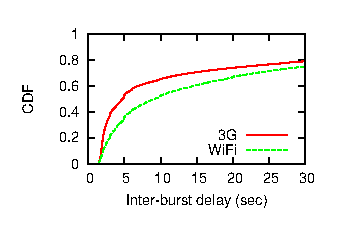
\includegraphics[width=.99\textwidth]{figures/mobisys12/burst_interval.eps}
\ncaption{\small CDF of Inter-burst delay for \UMICH~data set}
\label{fig:inter.burst}
	\end{minipage}
	\begin{minipage}[b]{.49\textwidth}
\centering
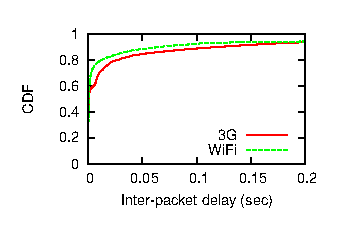
\includegraphics[width=.99\textwidth]{figures/mobisys12/packet_inter_delay.eps}
\ncaption{\small CDF of Inter-packet delay for \UMICH~data set}
\label{fig:inter.packet}
	\end{minipage}
\end{figure*}

To further understand the energy consumption, with the methodology discussed in \S\ref{sec:method.sim}, it is decomposed into promotion energy, data transfer energy, tail energy, and idle energy in Figure~\ref{fig:energy.breakdown} with results for aggregate analysis and 6 sample users. These energy values are calculated including the UE base power.

Promotion energy contributes to a small portion ($<4$\%) of the total energy for all networks, \ie in aggregate, its contribution is only 1.2\%, 2.5\% and 2.6\% for LTE, WiFi, and 3G, respectively. In terms of idle energy, WiFi has significantly higher percentage than LTE and 3G, despite small average power difference at idle state across networks, \ie 31.1mW~\footnote{The idle power for LTE network is calculated as the average power of a DRX cycle in \RI, and similarly for WiFi and 3G networks.} for LTE, 13.0mW for WiFi and 15.3mW for 3G. This is explained by WiFi's smaller total energy, making its idle energy contribution relatively higher.
%Since we assume that UE remains idle for the same time before complete sleep, total idle energy difference among different networks is also small. 

Aggregate data transfer energy percentage is 47.1\%, 42.1\% and 46.2\% for LTE, WiFi and 3G, respectively. The variation across users is high, \eg for LTE network, it ranges from 22.0\% to 62.3\%, due to traffic pattern differences across users.

Surprisingly, the biggest energy component for LTE network is tail, rather than data transfer. The average tail energy for LTE and 3G is 48.2\% and 48.1\% respectively compared to 7.2\% for WiFi. Our observation for 3G is consistent with previous study~\cite{imc.tailender}. Combined with high data transfer energy due to the higher power levels, tail energy lowers the energy efficiency of LTE and 3G compared to WiFi.


%Performance penalty: show a CDF of extra delay for all packets in WiFi/LTE networks.
%Evaluate the power saving, additional delay distribution on existing parameters and compare the ATT with Verizon if there is any difference.
%Break down into individual user and even individual app to understand the typical cause for I2A promotions (similar to Feng�s 3G study), and which parameter settings are better for what kind of traffic patterns.

\subsection{Impact of LTE parameters}
\label{sec:sim.parameter}

Similar to \S\ref{sec:sim.total}, we use WiFi traces in the \UMICH~data set to study the impact of LTE parameter configuration on radio energy $E$, channel scheduling delay $D$, and signaling overhead $S$. $E$ is the simulated total energy consumed by UE. Since most energy is consumed by radio interfaces, with display energy excluded, we approximate this total energy as radio energy. $D$ is the sum of scheduling delay for all packets, resulting from two factors: waiting for the next DRX cycle's on duration for a downlink packet and waiting for $T_{pro}$ during \RI~to \RC promotion. $S$ is the overhead of the LTE network for serving this UE. $S$ has different definitions in our study given that different parameters studied affect signaling load in different ways, \eg $T_{tail}$ affects mostly the state promotions, and $T_{pi}$ affects the total on duration in \RI. $D$ and $E$ directly affect end users via application delay and battery life time;  $S$ is of interest to cellular ISPs for supporting large user base at low cost.

\nsubsubsection{Impact of LTE tail timer $T_{tail}$}


In Figure~\ref{fig:ta2i}, we study the impact of LTE tail timer $T_{tail}$, with $S$ defined to be the total number of \RI~to \RC~promotions. $T_{tail}$ varies from 1 second to 30 seconds. $T_D$ is the default configuration of 11.58 seconds for $T_{tail}$ in the measured LTE network with the corresponding values of $E$, $D$ and $S$ calculated as $E_D$, $D_D$ and $S_D$, respectively. When $T_{tail}$ is set to be $T'$, similarly, we get $E'$, $D'$ and $S'$. The change relative to the default setting is calculated as $\Delta(E) = (E' - E_D) / E_D$, and similarly for $\Delta(D)$ and $\Delta(S)$. $\Delta$s for each $T_{tail}$ values are plotted in Figure~\ref{fig:ta2i} and they are all 0 at $T_D$.

As expected, a larger $T_{tail}$ value reduces both $D$ and $S$, at the cost of $E$.
We observe that $\Delta(S)$ and $\Delta(D)$ curves are almost identical, since most channel scheduling delay results from idle to active promotions. In addition, the impact of $T_{tail}$ on the radio energy $E$ is significant. For example, when $T_{tail}$ is set to be 30 seconds, total radio energy $E$ increases by 55\%, while for $T_{tail}=1$ second, $E$ decreases by 65\%, at the cost of 143\% $\Delta(D)$ and 169\% $\Delta(S)$. This indicates that $T_{tail}$ is a very important parameter for LTE network.


In previous study~\cite{mobisys.aro}, traffic bursts attribute to low efficiencies of radio resource and energy utilization in 3G UMTS network, due to tail time. Given that LTE has similar tail time, we analyze the bursts in the \UMICH data set. We follow the same definition of a {\sf burst} as in~\cite{mobisys.aro}, which is a sequence of consecutive packets whose inter-arrival time is less than a threshold $\delta$, with $\delta$ set to be 1.5 seconds, since it is longer than common cellular RTTs~\cite{mobisys.3gtest}. From ISP's perspective, $T_{tail}$ should not be smaller than majority of the inter-burst delays; otherwise, a larger number of promotions would be triggered. 

%We define a {\sf burst} $B$ to be a sequence of consecutive packets, $P_1, P_2, \cdots, P_n$, with ascending timestamps ($T_1 \leq T_{2} \leq \cdots \leq T_n$), such that for $1 \leq i \leq (n-1)$, $T_{i+1} - T_i \leq \Theta$, where $\Theta$ is the burst threshold empirically set to be 1.5 seconds, which is verified to have a negligible impact on our conclusions. Assume $P_0$ is the immediate packet before $P_1$ and $P_{n+1}$ is the immediate packet after $P_n$, we have $T_1 - T_0 > \Theta$ and $T_{n+1} - T_n > \Theta$, otherwise, $P_0$ or $P_{n+1}$ would belong to burst $B$.

We study the inter-burst delay in the 3G and WiFi traces of \UMICH~data set in Figure~\ref{fig:inter.burst}. For 3G traces, 67.3\% inter-burst delays are smaller than the default value of $T_{tail}$ (11.58 seconds), and 55.4\% for WiFi traces. Compared with WiFi traces, 3G traces have smaller inter-burst delays. We also observe the inter-burst delay distribution for different users have non-negligible differences. This makes us believe that a per-UE based dynamic $T_{tail}$ configuration mechanism, adapting to traffic patterns, provides a better chance for optimizing radio resource efficiency and balancing energy utilization. Notice that this approach is inside the radio access network and transparent to UE. Previous study on 3G UMTS network also points out two possible approaches to deal with the tail effect with support from UE, \ie applications proactively alter traffic patterns based on the state machine behavior without interaction with the network, or cooperate with the radio access network in allocating radio resources by fast dormancy~\cite{fast.dormancy.1, fast.dormancy.2}. These approaches remain to be applicable solutions for the tail problem in LTE.

%\comment{I don't see the differences of the two approaches: both require UE to adapt, what about the network adapts based on the UE behavior (UE specific timer settings)? please give citation.}

%Second, in general, small bursts are dominant, \ie 43.4\% bursts in 3G and 51.7\% bursts in WiFi has $\leq 100$ms burst length. Based on the burst duration CDF, the default setting of $T_{tail}$ covers 98.4\% bursts for 3G trace and 99.2\% bursts for WiFi trace in \UMICH. From this point of view, $T_{tail}$ is currently set to be a conservative and high value, if we simply consider burst coverage. A range between 5 seconds and 15 seconds is reasonable, and if $T_{tail}$ is set to be less than 5 seconds, we would see a sharp increase in the number of bursts that the tail fails to cover. However, there is no simple conclusion on which value is ``optimal'' for $T_{tail}$ and similarly for other parameters, depending on the system goals and requirements. 

\nsubsubsection{Impact of DRX inactivity timer $T_i$}

Figure~\ref{fig:t1} shows the tradeoff of setting DRX inactivity timer $T_i$. Signaling overhead $S$ is defined as the sum of the continuous reception time and DRX on durations in \RC, since during these time slots, UE exchanges control messages with eNB (base station of LTE network)~\cite{4gbook}. A larger $T_i$ keeps UE in continuous reception longer and reduces the scheduling delay for downlink packets, \ie no DRX waiting time, at the cost of higher energy usage, since continuous reception has higher power level than DRX idle state. $T_D$ is the default value 100ms.

We observe that $T_i$ has negligible impact on $E$, with only 2\% $\Delta(E)$ as $T_i$ is set to be 1 second. Different from $E$, $S$ is significantly affected by $T_i$.
For $D$, when $T_i$ is set to be small than 100ms, $\Delta(D)$ grows up to 80\%. However, even when $T_i$ is set to be as large as 1 second, $D$ is only reduced by 16\%. This can be partly explained by Figure~\ref{fig:inter.packet} that 88.6\% packet pairs has $\leq 100$ms inter-packet delay for 3G traces and 92.3\% for WiFi traces in the \UMICH~data set. Decreasing $T_i$ causes more packets arrive outside of continuous reception, which may experience DRX delay. Hence similar to $T_{tail}$, the setting of $T_i$ is also affected by the traffic pattern, \ie inter-packet delay distribution, which may differ across users.

%$T_i$ should not be set to be less than 25ms to prevent a large number of packets from experiencing DRX delay.% (Figure~\ref{fig:inter.packet}).

\nsubsubsection{Impact of DRX cycle in \RCB}

In \RC, Short DRX cycle timer $T_{is}$ determines the transition from Short DRX to Long DRX. Given that we already vary the DRX cycle to understand its impact, for simplicity, we assume $T_{is}$ to be 0, \ie the DRX cycle in \RC~refers to Long DRX cycle $T_{pl}$.

In Figure~\ref{fig:tpl}, $S$ is defined similarly as in Figure~\ref{fig:t1}, \ie the sum of continuous reception time and DRX on durations. $T_D$ is 40ms, the default setting for $T_{pl}$. First, we notice that compared with $T_D$, when $T_{pl}$ is set to be 100ms, energy saving $\Delta(E)$ is minor (0.2\%) with 13.0\% reduction in $S$, at the cost of 40\% increase in $D$. So $T_{pl}$ is not recommended to be set much higher than $T_D$ unless ISP prioritizes $S$ reduction.  When $T_{pl}$ is set to be a small value, for example 2ms, $E$ increases by 21.9\% and $D$ reduces by 18.1\%, with a significant increase in $S$ of 412.9\%. Especially for ISPs with fast growing LTE user volume and congested radio access network, DRX cycle in \RC~is not recommend to be set to too small values. We omit the simulation results for Short DRX cycle $T_{ps}$ and Short DRX timer $T_{is}$, since reducing $T_{ps}$ or increasing $T_{is}$ has similar effect of decreasing $T_{pl}$, \ie resulting in a shorter average DRX cycle, and their impact is similar as in Figure~\ref{fig:tpl}.

\subsubsection{Impact of DRX cycle in \RIB}

Similarly to \RC, we study the impact of DRX cycle in \RI. Under this setting, signaling overhead $S$ is defined to be the total on duration of DRX cycles in \RI, during which control messages are exchanged between UE and eNB~\cite{4gbook}. In Figure~\ref{fig:tpi}, the default setting 1.28s is shown as $T_D$. The impact of $T_{pi}$ on $E$ is not significant when $T_{pi}$ is larger than $T_D$, with 0.7\% energy saving when $T_{pi}$ set to be 2.0s, which also brings in 21.3\% increase in $D$ and 31.7\% reduction in $S$. When $T_{pi}$ is set to be 100ms, the energy overhead is 26.2\%, with 40.7\% reduction in $D$ and up to 1147.2\% increase in $S$.

Similar to $T_{pl}$, $T_{pi}$ causes significant signaling overhead when set to be too small. Default values for both $T_{pl}$ and $T_{pi}$ are reasonable settings and adjustment around the default configurations results in moderate impact on channel scheduling delay and negligible impact on radio energy.

In this section, we observe that LTE consumes up to 23 times the total energy of WiFi in the simulation, and the tail problem in 3G UMTS network is still a key contributor for the low energy efficiency for LTE. Similar to 3G network, $T_{tail}$ remains a key parameter for LTE. In addition to the UE-participated approaches including proactive traffic shaping and fast dormancy proposed by previous study~\cite{imc.3g}, we discuss a possible approach to solve the tail problem in LTE network, which dynamically adapts $T_{tail}$ to traffic pattern at a per-UE base, being transparent to UE. Similar observations are shared by the other LTE parameters and we leave the feasibility study of such dynamic parameter configuration framework for LTE as future work.

%\comment{give citation?  I thought Feng's work--ToP also proposed this.} TOP does not include this approach
%\comment{summarize highlight findings. recommendation adjust parameters, reference 3G optimization papers. UE adapts to network, and network adapts to network. fast dormancy for LTE should cite. (will check fast dormancy spec does it say LTE?)}


%\comment{study the overhead of On Duration}

%New policies to evaluate (baseline is assuming that when network is completely aware of all the user packet patterns):
%\begin{itemize}
%\item A fixed but maybe better configuration by looking at all users� traffic patters? Need to compare traffic pattern similarities across all users. Supposedly, big diversity!
%\item Adaptive policy per user (DRX setting adapt to each user�s last X seconds or last N packets, etc.)
%\comment{point out the energy ratio is less when we tune parameter timer to be ...}
%\end{itemize}
